% Slide 8 | Results E5 | M2 (Nitin Sureshkumar) | 2:00 | headline backtest on US stocks
\begin{frame}{E5: US stocks, no rule is significant}
\framesubtitle{Slide 8 \textbullet\ Results E5 \textbullet\ M2 \textbullet\ 2:00}
\vspace{-2pt}
\begin{columns}[T,onlytextwidth]
\column{0.46\textwidth}
  \footnotesize\setlength{\tabcolsep}{4pt}
  \begin{tabular}{@{}lrr@{}}
    \toprule
    Rule & Return \%/yr & Sharpe (SE) \\
    \midrule
    S0 Distance & $-0.09$ & $-0.05$ (0.25) \\
    S1 z-score  & 0.33 & \textbf{0.19} (0.25) \\
    S2 s-score  & 0.10 & 0.06 (0.25) \\
    S3 Bertram  & 0.12 & 0.06 (0.25) \\
    \bottomrule
  \end{tabular}\\[3pt]
  {\scriptsize 56 large caps in 7 sectors, 2010--2026, 10 bp}\\[5pt]
  \small\raggedright
  \begin{itemize}\setlength{\itemsep}{2pt}
    \item S1 earns about 44 bp per trade before costs
    \item but 28--45\% of trades never close ($\approx -3\%$ each)
  \end{itemize}
\column{0.50\textwidth}
  \centering
  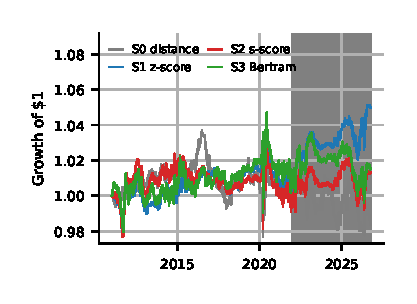
\includegraphics[width=\linewidth]{fig_e5_cumulative_report}
\end{columns}
\pairTakeaway{Only about 8 of 196 candidate pairs pass the test, no more than chance.}
\end{frame}
